\documentclass[1p]{elsarticle_modified}
%\bibliographystyle{elsarticle-num}

%\usepackage[colorlinks]{hyperref}
%\usepackage{abbrmath_seonhwa} %\Abb, \Ascr, \Acal ,\Abf, \Afrak
\usepackage{amsfonts}
\usepackage{amssymb}
\usepackage{amsmath}
\usepackage{amsthm}
\usepackage{scalefnt}
\usepackage{amsbsy}
\usepackage{kotex}
\usepackage{caption}
\usepackage{subfig}
\usepackage{color}
\usepackage{graphicx}
\usepackage{xcolor} %% white, black, red, green, blue, cyan, magenta, yellow
\usepackage{float}
\usepackage{setspace}
\usepackage{hyperref}

\usepackage{tikz}
\usetikzlibrary{arrows}

\usepackage{multirow}
\usepackage{array} % fixed length table
\usepackage{hhline}

%%%%%%%%%%%%%%%%%%%%%
\makeatletter
\renewcommand*\env@matrix[1][\arraystretch]{%
	\edef\arraystretch{#1}%
	\hskip -\arraycolsep
	\let\@ifnextchar\new@ifnextchar
	\array{*\c@MaxMatrixCols c}}
\makeatother %https://tex.stackexchange.com/questions/14071/how-can-i-increase-the-line-spacing-in-a-matrix
%%%%%%%%%%%%%%%

\usepackage[normalem]{ulem}

\newcommand{\msout}[1]{\ifmmode\text{\sout{\ensuremath{#1}}}\else\sout{#1}\fi}
%SOURCE: \msout is \stkout macro in https://tex.stackexchange.com/questions/20609/strikeout-in-math-mode

\newcommand{\cancel}[1]{
	\ifmmode
	{\color{red}\msout{#1}}
	\else
	{\color{red}\sout{#1}}
	\fi
}

\newcommand{\add}[1]{
	{\color{blue}\uwave{#1}}
}

\newcommand{\replace}[2]{
	\ifmmode
	{\color{red}\msout{#1}}{\color{blue}\uwave{#2}}
	\else
	{\color{red}\sout{#1}}{\color{blue}\uwave{#2}}
	\fi
}

\newcommand{\Sol}{\mathcal{S}} %segment
\newcommand{\D}{D} %diagram
\newcommand{\A}{\mathcal{A}} %arc


%%%%%%%%%%%%%%%%%%%%%%%%%%%%%5 test

\def\sl{\operatorname{\textup{SL}}(2,\Cbb)}
\def\psl{\operatorname{\textup{PSL}}(2,\Cbb)}
\def\quan{\mkern 1mu \triangleright \mkern 1mu}

\theoremstyle{definition}
\newtheorem{thm}{Theorem}[section]
\newtheorem{prop}[thm]{Proposition}
\newtheorem{lem}[thm]{Lemma}
\newtheorem{ques}[thm]{Question}
\newtheorem{cor}[thm]{Corollary}
\newtheorem{defn}[thm]{Definition}
\newtheorem{exam}[thm]{Example}
\newtheorem{rmk}[thm]{Remark}
\newtheorem{alg}[thm]{Algorithm}

\newcommand{\I}{\sqrt{-1}}
\begin{document}

%\begin{frontmatter}
%
%\title{Boundary parabolic representations of knots up to 8 crossings}
%
%%% Group authors per affiliation:
%\author{Yunhi Cho} 
%\address{Department of Mathematics, University of Seoul, Seoul, Korea}
%\ead{yhcho@uos.ac.kr}
%
%
%\author{Seonhwa Kim} %\fnref{s_kim}}
%\address{Center for Geometry and Physics, Institute for Basic Science, Pohang, 37673, Korea}
%\ead{ryeona17@ibs.re.kr}
%
%\author{Hyuk Kim}
%\address{Department of Mathematical Sciences, Seoul National University, Seoul 08826, Korea}
%\ead{hyukkim@snu.ac.kr}
%
%\author{Seokbeom Yoon}
%\address{Department of Mathematical Sciences, Seoul National University, Seoul, 08826,  Korea}
%\ead{sbyoon15@snu.ac.kr}
%
%\begin{abstract}
%We find all boundary parabolic representation of knots up to 8 crossings.
%
%\end{abstract}
%\begin{keyword}
%    \MSC[2010] 57M25 
%\end{keyword}
%
%\end{frontmatter}

%\linenumbers
%\tableofcontents
%
\newcommand\colored[1]{\textcolor{white}{\rule[-0.35ex]{0.8em}{1.4ex}}\kern-0.8em\color{red} #1}%
%\newcommand\colored[1]{\textcolor{white}{ #1}\kern-2.17ex	\textcolor{white}{ #1}\kern-1.81ex	\textcolor{white}{ #1}\kern-2.15ex\color{red}#1	}

{\Large $\underline{12a_{0525}~(K12a_{0525})}$}

\setlength{\tabcolsep}{10pt}
\renewcommand{\arraystretch}{1.6}
\vspace{1cm}\begin{tabular}{m{100pt}>{\centering\arraybackslash}m{274pt}}
\multirow{5}{120pt}{
	\centering
	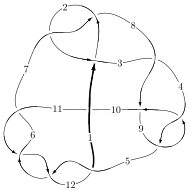
\includegraphics[width=112pt]{../../../GIT/diagram.site/Diagrams/png/1326_12a_0525.png}\\
\ \ \ A knot diagram\footnotemark}&
\allowdisplaybreaks
\textbf{Linearized knot diagam} \\
\cline{2-2}
 &
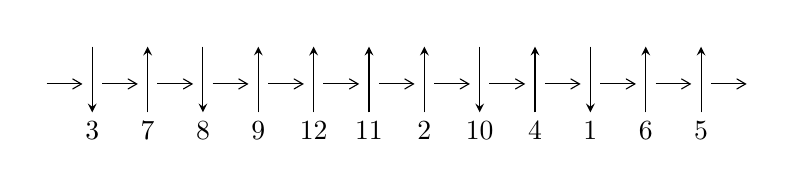
\begin{tikzpicture}[x=20pt, y=17pt]
	% nodes
	\node (C0) at (0, 0) {};
	\node (C1) at (1, 0) {};
	\node (C1U) at (1, +1) {};
	\node (C1D) at (1, -1) {3};

	\node (C2) at (2, 0) {};
	\node (C2U) at (2, +1) {};
	\node (C2D) at (2, -1) {7};

	\node (C3) at (3, 0) {};
	\node (C3U) at (3, +1) {};
	\node (C3D) at (3, -1) {8};

	\node (C4) at (4, 0) {};
	\node (C4U) at (4, +1) {};
	\node (C4D) at (4, -1) {9};

	\node (C5) at (5, 0) {};
	\node (C5U) at (5, +1) {};
	\node (C5D) at (5, -1) {12};

	\node (C6) at (6, 0) {};
	\node (C6U) at (6, +1) {};
	\node (C6D) at (6, -1) {11};

	\node (C7) at (7, 0) {};
	\node (C7U) at (7, +1) {};
	\node (C7D) at (7, -1) {2};

	\node (C8) at (8, 0) {};
	\node (C8U) at (8, +1) {};
	\node (C8D) at (8, -1) {10};

	\node (C9) at (9, 0) {};
	\node (C9U) at (9, +1) {};
	\node (C9D) at (9, -1) {4};

	\node (C10) at (10, 0) {};
	\node (C10U) at (10, +1) {};
	\node (C10D) at (10, -1) {1};

	\node (C11) at (11, 0) {};
	\node (C11U) at (11, +1) {};
	\node (C11D) at (11, -1) {6};

	\node (C12) at (12, 0) {};
	\node (C12U) at (12, +1) {};
	\node (C12D) at (12, -1) {5};
	\node (C13) at (13, 0) {};

	% arrows
	\draw[->,>={angle 60}]
	(C0) edge (C1) (C1) edge (C2) (C2) edge (C3) (C3) edge (C4) (C4) edge (C5) (C5) edge (C6) (C6) edge (C7) (C7) edge (C8) (C8) edge (C9) (C9) edge (C10) (C10) edge (C11) (C11) edge (C12) (C12) edge (C13) ;	\draw[->,>=stealth]
	(C1U) edge (C1D) (C2D) edge (C2U) (C3U) edge (C3D) (C4D) edge (C4U) (C5D) edge (C5U) (C6D) edge (C6U) (C7D) edge (C7U) (C8U) edge (C8D) (C9D) edge (C9U) (C10U) edge (C10D) (C11D) edge (C11U) (C12D) edge (C12U) ;
	\end{tikzpicture} \\
\hhline{~~} \\& 
\textbf{Solving Sequence} \\ \cline{2-2} 
 &
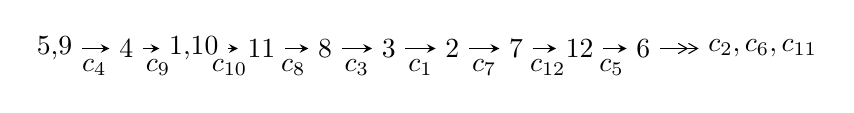
\begin{tikzpicture}[x=23pt, y=7pt]
	% node
	\node (A0) at (-1/8, 0) {5,9};
	\node (A1) at (1, 0) {4};
	\node (A2) at (33/16, 0) {1,10};
	\node (A3) at (25/8, 0) {11};
	\node (A4) at (33/8, 0) {8};
	\node (A5) at (41/8, 0) {3};
	\node (A6) at (49/8, 0) {2};
	\node (A7) at (57/8, 0) {7};
	\node (A8) at (65/8, 0) {12};
	\node (A9) at (73/8, 0) {6};
	\node (C1) at (1/2, -1) {$c_{4}$};
	\node (C2) at (3/2, -1) {$c_{9}$};
	\node (C3) at (21/8, -1) {$c_{10}$};
	\node (C4) at (29/8, -1) {$c_{8}$};
	\node (C5) at (37/8, -1) {$c_{3}$};
	\node (C6) at (45/8, -1) {$c_{1}$};
	\node (C7) at (53/8, -1) {$c_{7}$};
	\node (C8) at (61/8, -1) {$c_{12}$};
	\node (C9) at (69/8, -1) {$c_{5}$};
	\node (A10) at (11, 0) {$c_{2},c_{6},c_{11}$};

	% edge
	\draw[->,>=stealth]	
	(A0) edge (A1) (A1) edge (A2) (A2) edge (A3) (A3) edge (A4) (A4) edge (A5) (A5) edge (A6) (A6) edge (A7) (A7) edge (A8) (A8) edge (A9) ;
	\draw[->>,>={angle 60}]	
	(A9) edge (A10);
\end{tikzpicture} \\ 

\end{tabular} \\

\footnotetext{
The image of knot diagram is generated by the software ``\textbf{Draw programme}" developed by Andrew Bartholomew(\url{http://www.layer8.co.uk/maths/draw/index.htm\#Running-draw}), where we modified some parts for our purpose(\url{https://github.com/CATsTAILs/LinksPainter}).
}\phantom \\ \newline 
\centering \textbf{Ideals for irreducible components\footnotemark of $X_{\text{par}}$} 
 
\begin{align*}
I^u_{1}&=\langle 
- u^{27}+u^{26}+\cdots+4 b+1,\;u^{27}- u^{26}+\cdots+4 a+3,\;u^{28}+7 u^{26}+\cdots+u+1\rangle \\
I^u_{2}&=\langle 
716399893584 u^{45}+1564714832102 u^{44}+\cdots+14311443700915 b-42121557729620,\\
\phantom{I^u_{2}}&\phantom{= \langle  }-1246408210566 u^{45}-1464820132004 u^{44}+\cdots+14311443700915 a-50730055068599,\\
\phantom{I^u_{2}}&\phantom{= \langle  }u^{46}- u^{45}+\cdots-6 u+5\rangle \\
I^u_{3}&=\langle 
b+a+1,\;a^2+a u+2 a+u+2,\;u^2+1\rangle \\
\\
\end{align*}
\raggedright * 3 irreducible components of $\dim_{\mathbb{C}}=0$, with total 78 representations.\\
\footnotetext{All coefficients of polynomials are rational numbers. But the coefficients are sometimes approximated in decimal forms when there is not enough margin.}
\newpage
\renewcommand{\arraystretch}{1}
\centering \section*{I. $I^u_{1}= \langle - u^{27}+u^{26}+\cdots+4 b+1,\;u^{27}- u^{26}+\cdots+4 a+3,\;u^{28}+7 u^{26}+\cdots+u+1 \rangle$}
\flushleft \textbf{(i) Arc colorings}\\
\begin{tabular}{m{7pt} m{180pt} m{7pt} m{180pt} }
\flushright $a_{5}=$&$\begin{pmatrix}1\\0\end{pmatrix}$ \\
\flushright $a_{9}=$&$\begin{pmatrix}0\\u\end{pmatrix}$ \\
\flushright $a_{4}=$&$\begin{pmatrix}1\\u^2\end{pmatrix}$ \\
\flushright $a_{1}=$&$\begin{pmatrix}-\frac{1}{4} u^{27}+\frac{1}{4} u^{26}+\cdots-\frac{1}{2} u^4-\frac{3}{4}\\\frac{1}{4} u^{27}-\frac{1}{4} u^{26}+\cdots- u^2-\frac{1}{4}\end{pmatrix}$ \\
\flushright $a_{10}=$&$\begin{pmatrix}u\\u^3+u\end{pmatrix}$ \\
\flushright $a_{11}=$&$\begin{pmatrix}\frac{5}{4} u^{27}+\frac{3}{4} u^{26}+\cdots+3 u+\frac{5}{4}\\- u^{27}-\frac{1}{2} u^{26}+\cdots-\frac{3}{2} u-1\end{pmatrix}$ \\
\flushright $a_{8}=$&$\begin{pmatrix}u^3\\u^5+u^3+u\end{pmatrix}$ \\
\flushright $a_{3}=$&$\begin{pmatrix}- u^6- u^4+1\\- u^8-2 u^6-2 u^4\end{pmatrix}$ \\
\flushright $a_{2}=$&$\begin{pmatrix}-\frac{1}{4} u^{27}+\frac{1}{4} u^{26}+\cdots+u^2-\frac{3}{4}\\\frac{1}{4} u^{27}-\frac{1}{4} u^{26}+\cdots- u^2-\frac{1}{4}\end{pmatrix}$ \\
\flushright $a_{7}=$&$\begin{pmatrix}\frac{1}{4} u^{27}+\frac{1}{4} u^{26}+\cdots-\frac{1}{2} u+\frac{1}{4}\\-\frac{1}{4} u^{27}-\frac{1}{4} u^{26}+\cdots+\frac{1}{2} u-\frac{1}{4}\end{pmatrix}$ \\
\flushright $a_{12}=$&$\begin{pmatrix}-\frac{1}{2} u^{27}+\frac{1}{2} u^{26}+\cdots+u^2-\frac{1}{2}\\\frac{1}{4} u^{27}-\frac{1}{4} u^{26}+\cdots- u^2-\frac{1}{4}\end{pmatrix}$ \\
\flushright $a_{6}=$&$\begin{pmatrix}\frac{5}{4} u^{27}-\frac{5}{4} u^{26}+\cdots-\frac{5}{2} u^4-\frac{5}{4}\\-\frac{1}{2} u^{27}+\frac{1}{2} u^{26}+\cdots-\frac{1}{2} u^2+1\end{pmatrix}$\\&\end{tabular}
\flushleft \textbf{(ii) Obstruction class $= -1$}\\~\\
\flushleft \textbf{(iii) Cusp Shapes $= 6 u^{27}-3 u^{26}+41 u^{25}-15 u^{24}+144 u^{23}-42 u^{22}+311 u^{21}-64 u^{20}+447 u^{19}-54 u^{18}+417 u^{17}+12 u^{16}+224 u^{15}+72 u^{14}+22 u^{13}+88 u^{12}-43 u^{11}+23 u^{10}-15 u^8+40 u^7-32 u^6+39 u^5-2 u^4+15 u^3+u+2$}\\~\\
\newpage\renewcommand{\arraystretch}{1}
\flushleft \textbf{(iv) u-Polynomials at the component}\newline \\
\begin{tabular}{m{50pt}|m{274pt}}
Crossings & \hspace{64pt}u-Polynomials at each crossing \\
\hline $$\begin{aligned}c_{1},c_{8}\end{aligned}$$&$\begin{aligned}
&u^{28}+14 u^{27}+\cdots+3 u+1
\end{aligned}$\\
\hline $$\begin{aligned}c_{2},c_{4},c_{7}\\c_{9}\end{aligned}$$&$\begin{aligned}
&u^{28}+7 u^{26}+\cdots- u+1
\end{aligned}$\\
\hline $$\begin{aligned}c_{3}\end{aligned}$$&$\begin{aligned}
&u^{28}-3 u^{27}+\cdots-16 u+32
\end{aligned}$\\
\hline $$\begin{aligned}c_{5},c_{6},c_{11}\\c_{12}\end{aligned}$$&$\begin{aligned}
&u^{28}-3 u^{27}+\cdots-11 u+2
\end{aligned}$\\
\hline $$\begin{aligned}c_{10}\end{aligned}$$&$\begin{aligned}
&u^{28}-9 u^{27}+\cdots-577 u+88
\end{aligned}$\\
\hline
\end{tabular}\\~\\
\newpage\renewcommand{\arraystretch}{1}
\flushleft \textbf{(v) Riley Polynomials at the component}\newline \\
\begin{tabular}{m{50pt}|m{274pt}}
Crossings & \hspace{64pt}Riley Polynomials at each crossing \\
\hline $$\begin{aligned}c_{1},c_{8}\end{aligned}$$&$\begin{aligned}
&y^{28}+6 y^{27}+\cdots+7 y+1
\end{aligned}$\\
\hline $$\begin{aligned}c_{2},c_{4},c_{7}\\c_{9}\end{aligned}$$&$\begin{aligned}
&y^{28}+14 y^{27}+\cdots+3 y+1
\end{aligned}$\\
\hline $$\begin{aligned}c_{3}\end{aligned}$$&$\begin{aligned}
&y^{28}-17 y^{27}+\cdots+9472 y+1024
\end{aligned}$\\
\hline $$\begin{aligned}c_{5},c_{6},c_{11}\\c_{12}\end{aligned}$$&$\begin{aligned}
&y^{28}+33 y^{27}+\cdots- y+4
\end{aligned}$\\
\hline $$\begin{aligned}c_{10}\end{aligned}$$&$\begin{aligned}
&y^{28}-15 y^{27}+\cdots-37601 y+7744
\end{aligned}$\\
\hline
\end{tabular}\\~\\
\newpage\flushleft \textbf{(vi) Complex Volumes and Cusp Shapes}
$$\begin{array}{c|c|c}  
\text{Solutions to }I^u_{1}& \I (\text{vol} + \sqrt{-1}CS) & \text{Cusp shape}\\
 \hline 
\begin{aligned}
u &= -0.561145 + 0.801172 I \\
a &= \phantom{-}0.789871 + 0.574150 I \\
b &= \phantom{-}0.517508 + 0.330068 I\end{aligned}
 & \phantom{-}1.48439 - 2.80149 I & \phantom{-}6.48594 + 3.23788 I \\ \hline\begin{aligned}
u &= -0.561145 - 0.801172 I \\
a &= \phantom{-}0.789871 - 0.574150 I \\
b &= \phantom{-}0.517508 - 0.330068 I\end{aligned}
 & \phantom{-}1.48439 + 2.80149 I & \phantom{-}6.48594 - 3.23788 I \\ \hline\begin{aligned}
u &= \phantom{-}0.579647 + 0.897152 I \\
a &= \phantom{-}1.50711 - 0.28805 I \\
b &= \phantom{-}0.497793 + 0.554969 I\end{aligned}
 & \phantom{-}0.84370 + 6.32564 I & \phantom{-}3.80658 - 10.10200 I \\ \hline\begin{aligned}
u &= \phantom{-}0.579647 - 0.897152 I \\
a &= \phantom{-}1.50711 + 0.28805 I \\
b &= \phantom{-}0.497793 - 0.554969 I\end{aligned}
 & \phantom{-}0.84370 - 6.32564 I & \phantom{-}3.80658 + 10.10200 I \\ \hline\begin{aligned}
u &= \phantom{-}0.644615 + 0.631322 I \\
a &= -0.490860 - 1.215860 I \\
b &= \phantom{-}0.02723 - 1.47847 I\end{aligned}
 & -4.08922 + 1.25049 I & \phantom{-}3.66147 - 3.30700 I \\ \hline\begin{aligned}
u &= \phantom{-}0.644615 - 0.631322 I \\
a &= -0.490860 + 1.215860 I \\
b &= \phantom{-}0.02723 + 1.47847 I\end{aligned}
 & -4.08922 - 1.25049 I & \phantom{-}3.66147 + 3.30700 I \\ \hline\begin{aligned}
u &= -0.215428 + 0.829791 I \\
a &= -0.37664 - 1.75550 I \\
b &= \phantom{-}0.01632 + 1.64841 I\end{aligned}
 & -11.32300 - 1.08394 I & -0.67442 + 6.46054 I \\ \hline\begin{aligned}
u &= -0.215428 - 0.829791 I \\
a &= -0.37664 + 1.75550 I \\
b &= \phantom{-}0.01632 - 1.64841 I\end{aligned}
 & -11.32300 + 1.08394 I & -0.67442 - 6.46054 I \\ \hline\begin{aligned}
u &= -0.605441 + 0.975082 I \\
a &= \phantom{-}2.03396 - 0.23377 I \\
b &= \phantom{-}0.12308 - 1.53651 I\end{aligned}
 & -6.10857 - 8.52011 I & \phantom{-}0.08752 + 8.22687 I \\ \hline\begin{aligned}
u &= -0.605441 - 0.975082 I \\
a &= \phantom{-}2.03396 + 0.23377 I \\
b &= \phantom{-}0.12308 + 1.53651 I\end{aligned}
 & -6.10857 + 8.52011 I & \phantom{-}0.08752 - 8.22687 I\\
 \hline 
 \end{array}$$\newpage$$\begin{array}{c|c|c}  
\text{Solutions to }I^u_{1}& \I (\text{vol} + \sqrt{-1}CS) & \text{Cusp shape}\\
 \hline 
\begin{aligned}
u &= -0.810575 + 0.181460 I \\
a &= -1.099550 - 0.535592 I \\
b &= -0.11876 - 1.60426 I\end{aligned}
 & -8.19035 + 4.61598 I & \phantom{-}1.91466 - 2.19636 I \\ \hline\begin{aligned}
u &= -0.810575 - 0.181460 I \\
a &= -1.099550 + 0.535592 I \\
b &= -0.11876 + 1.60426 I\end{aligned}
 & -8.19035 - 4.61598 I & \phantom{-}1.91466 + 2.19636 I \\ \hline\begin{aligned}
u &= \phantom{-}0.300734 + 0.727001 I \\
a &= -0.319517 + 0.635052 I \\
b &= \phantom{-}0.051371 - 0.848410 I\end{aligned}
 & -2.65911 + 1.36971 I & -0.64034 - 4.77051 I \\ \hline\begin{aligned}
u &= \phantom{-}0.300734 - 0.727001 I \\
a &= -0.319517 - 0.635052 I \\
b &= \phantom{-}0.051371 + 0.848410 I\end{aligned}
 & -2.65911 - 1.36971 I & -0.64034 + 4.77051 I \\ \hline\begin{aligned}
u &= -0.472666 + 1.163270 I \\
a &= \phantom{-}0.025330 + 0.342893 I \\
b &= -0.373723 - 0.874275 I\end{aligned}
 & -7.17751 - 5.06879 I & -3.79171 + 3.11845 I \\ \hline\begin{aligned}
u &= -0.472666 - 1.163270 I \\
a &= \phantom{-}0.025330 - 0.342893 I \\
b &= -0.373723 + 0.874275 I\end{aligned}
 & -7.17751 + 5.06879 I & -3.79171 - 3.11845 I \\ \hline\begin{aligned}
u &= \phantom{-}0.434237 + 1.181820 I \\
a &= \phantom{-}0.271152 - 1.262610 I \\
b &= -0.09543 + 1.65532 I\end{aligned}
 & -15.9103 + 3.3004 I & -5.83767 - 4.22098 I \\ \hline\begin{aligned}
u &= \phantom{-}0.434237 - 1.181820 I \\
a &= \phantom{-}0.271152 + 1.262610 I \\
b &= -0.09543 - 1.65532 I\end{aligned}
 & -15.9103 - 3.3004 I & -5.83767 + 4.22098 I \\ \hline\begin{aligned}
u &= \phantom{-}0.711695 + 0.202130 I \\
a &= -1.179690 + 0.185635 I \\
b &= -0.417783 + 0.681445 I\end{aligned}
 & -0.38114 - 2.62748 I & \phantom{-}4.50546 + 4.03150 I \\ \hline\begin{aligned}
u &= \phantom{-}0.711695 - 0.202130 I \\
a &= -1.179690 - 0.185635 I \\
b &= -0.417783 - 0.681445 I\end{aligned}
 & -0.38114 + 2.62748 I & \phantom{-}4.50546 - 4.03150 I\\
 \hline 
 \end{array}$$\newpage$$\begin{array}{c|c|c}  
\text{Solutions to }I^u_{1}& \I (\text{vol} + \sqrt{-1}CS) & \text{Cusp shape}\\
 \hline 
\begin{aligned}
u &= \phantom{-}0.517461 + 1.173180 I \\
a &= -0.528302 + 0.520595 I \\
b &= -0.642923 + 0.090809 I\end{aligned}
 & -4.19208 + 8.45490 I & \phantom{-}1.37879 - 5.98873 I \\ \hline\begin{aligned}
u &= \phantom{-}0.517461 - 1.173180 I \\
a &= -0.528302 - 0.520595 I \\
b &= -0.642923 - 0.090809 I\end{aligned}
 & -4.19208 - 8.45490 I & \phantom{-}1.37879 + 5.98873 I \\ \hline\begin{aligned}
u &= -0.532917 + 1.201560 I \\
a &= -1.37394 - 0.82619 I \\
b &= -0.498601 + 0.771418 I\end{aligned}
 & -6.21060 - 12.29660 I & -2.15740 + 10.05358 I \\ \hline\begin{aligned}
u &= -0.532917 - 1.201560 I \\
a &= -1.37394 + 0.82619 I \\
b &= -0.498601 - 0.771418 I\end{aligned}
 & -6.21060 + 12.29660 I & -2.15740 - 10.05358 I \\ \hline\begin{aligned}
u &= \phantom{-}0.539110 + 1.224760 I \\
a &= -2.19344 + 0.93037 I \\
b &= -0.14542 - 1.63022 I\end{aligned}
 & -14.3989 + 14.7396 I & -4.25699 - 8.49623 I \\ \hline\begin{aligned}
u &= \phantom{-}0.539110 - 1.224760 I \\
a &= -2.19344 - 0.93037 I \\
b &= -0.14542 + 1.63022 I\end{aligned}
 & -14.3989 - 14.7396 I & -4.25699 + 8.49623 I \\ \hline\begin{aligned}
u &= -0.529327 + 0.333044 I \\
a &= -1.065480 + 0.149372 I \\
b &= -0.440655 + 0.212109 I\end{aligned}
 & \phantom{-}1.000800 - 0.418896 I & \phantom{-}9.51810 + 3.62447 I \\ \hline\begin{aligned}
u &= -0.529327 - 0.333044 I \\
a &= -1.065480 - 0.149372 I \\
b &= -0.440655 - 0.212109 I\end{aligned}
 & \phantom{-}1.000800 + 0.418896 I & \phantom{-}9.51810 - 3.62447 I\\
 \hline 
 \end{array}$$\newpage\newpage\renewcommand{\arraystretch}{1}
\centering \section*{II. $I^u_{2}= \langle 7.16\times10^{11} u^{45}+1.56\times10^{12} u^{44}+\cdots+1.43\times10^{13} b-4.21\times10^{13},\;-1.25\times10^{12} u^{45}-1.46\times10^{12} u^{44}+\cdots+1.43\times10^{13} a-5.07\times10^{13},\;u^{46}- u^{45}+\cdots-6 u+5 \rangle$}
\flushleft \textbf{(i) Arc colorings}\\
\begin{tabular}{m{7pt} m{180pt} m{7pt} m{180pt} }
\flushright $a_{5}=$&$\begin{pmatrix}1\\0\end{pmatrix}$ \\
\flushright $a_{9}=$&$\begin{pmatrix}0\\u\end{pmatrix}$ \\
\flushright $a_{4}=$&$\begin{pmatrix}1\\u^2\end{pmatrix}$ \\
\flushright $a_{1}=$&$\begin{pmatrix}0.0870917 u^{45}+0.102353 u^{44}+\cdots+0.144487 u+3.54472\\-0.0500578 u^{45}-0.109333 u^{44}+\cdots+1.16384 u+2.94321\end{pmatrix}$ \\
\flushright $a_{10}=$&$\begin{pmatrix}u\\u^3+u\end{pmatrix}$ \\
\flushright $a_{11}=$&$\begin{pmatrix}-0.326284 u^{45}+0.410432 u^{44}+\cdots-4.06775 u+1.72544\\0.543037 u^{45}+0.187376 u^{44}+\cdots-0.175104 u-4.56461\end{pmatrix}$ \\
\flushright $a_{8}=$&$\begin{pmatrix}u^3\\u^5+u^3+u\end{pmatrix}$ \\
\flushright $a_{3}=$&$\begin{pmatrix}- u^6- u^4+1\\- u^8-2 u^6-2 u^4\end{pmatrix}$ \\
\flushright $a_{2}=$&$\begin{pmatrix}0.343127 u^{45}+0.178658 u^{44}+\cdots-0.482261 u+2.67882\\-0.517669 u^{45}+0.00968254 u^{44}+\cdots+1.41813 u+3.82144\end{pmatrix}$ \\
\flushright $a_{7}=$&$\begin{pmatrix}-0.804906 u^{45}+1.05487 u^{44}+\cdots-5.92981 u+4.66531\\0.0268193 u^{45}-0.282855 u^{44}+\cdots-0.213286 u+0.465832\end{pmatrix}$ \\
\flushright $a_{12}=$&$\begin{pmatrix}0.137150 u^{45}+0.211686 u^{44}+\cdots-1.01935 u+0.601511\\-0.0500578 u^{45}-0.109333 u^{44}+\cdots+1.16384 u+2.94321\end{pmatrix}$ \\
\flushright $a_{6}=$&$\begin{pmatrix}0.159624 u^{45}+0.184010 u^{44}+\cdots-0.492668 u-5.14365\\-0.0612648 u^{45}-0.180573 u^{44}+\cdots+1.65763 u+0.574784\end{pmatrix}$\\&\end{tabular}
\flushleft \textbf{(ii) Obstruction class $= -1$}\\~\\
\flushleft \textbf{(iii) Cusp Shapes $= -\frac{26464957613496}{14311443700915} u^{45}+\frac{19226079710712}{14311443700915} u^{44}+\cdots-\frac{165615168368444}{14311443700915} u-\frac{9675043718942}{2862288740183}$}\\~\\
\newpage\renewcommand{\arraystretch}{1}
\flushleft \textbf{(iv) u-Polynomials at the component}\newline \\
\begin{tabular}{m{50pt}|m{274pt}}
Crossings & \hspace{64pt}u-Polynomials at each crossing \\
\hline $$\begin{aligned}c_{1},c_{8}\end{aligned}$$&$\begin{aligned}
&u^{46}+27 u^{45}+\cdots+44 u+25
\end{aligned}$\\
\hline $$\begin{aligned}c_{2},c_{4},c_{7}\\c_{9}\end{aligned}$$&$\begin{aligned}
&u^{46}+u^{45}+\cdots+6 u+5
\end{aligned}$\\
\hline $$\begin{aligned}c_{3}\end{aligned}$$&$\begin{aligned}
&(u^{23}+u^{22}+\cdots+4 u-5)^{2}
\end{aligned}$\\
\hline $$\begin{aligned}c_{5},c_{6},c_{11}\\c_{12}\end{aligned}$$&$\begin{aligned}
&(u^{23}+u^{22}+\cdots-2 u-1)^{2}
\end{aligned}$\\
\hline $$\begin{aligned}c_{10}\end{aligned}$$&$\begin{aligned}
&(u^{23}-7 u^{22}+\cdots+40 u-17)^{2}
\end{aligned}$\\
\hline
\end{tabular}\\~\\
\newpage\renewcommand{\arraystretch}{1}
\flushleft \textbf{(v) Riley Polynomials at the component}\newline \\
\begin{tabular}{m{50pt}|m{274pt}}
Crossings & \hspace{64pt}Riley Polynomials at each crossing \\
\hline $$\begin{aligned}c_{1},c_{8}\end{aligned}$$&$\begin{aligned}
&y^{46}-17 y^{45}+\cdots-11736 y+625
\end{aligned}$\\
\hline $$\begin{aligned}c_{2},c_{4},c_{7}\\c_{9}\end{aligned}$$&$\begin{aligned}
&y^{46}+27 y^{45}+\cdots+44 y+25
\end{aligned}$\\
\hline $$\begin{aligned}c_{3}\end{aligned}$$&$\begin{aligned}
&(y^{23}-17 y^{22}+\cdots-144 y-25)^{2}
\end{aligned}$\\
\hline $$\begin{aligned}c_{5},c_{6},c_{11}\\c_{12}\end{aligned}$$&$\begin{aligned}
&(y^{23}+27 y^{22}+\cdots-4 y-1)^{2}
\end{aligned}$\\
\hline $$\begin{aligned}c_{10}\end{aligned}$$&$\begin{aligned}
&(y^{23}-9 y^{22}+\cdots+1260 y-289)^{2}
\end{aligned}$\\
\hline
\end{tabular}\\~\\
\newpage\flushleft \textbf{(vi) Complex Volumes and Cusp Shapes}
$$\begin{array}{c|c|c}  
\text{Solutions to }I^u_{2}& \I (\text{vol} + \sqrt{-1}CS) & \text{Cusp shape}\\
 \hline 
\begin{aligned}
u &= \phantom{-}0.594093 + 0.867126 I \\
a &= -1.78487 - 0.73898 I \\
b &= -0.08584 - 1.50808 I\end{aligned}
 & -4.75454 + 3.53591 I & \phantom{-}2.63493 - 3.24061 I \\ \hline\begin{aligned}
u &= \phantom{-}0.594093 - 0.867126 I \\
a &= -1.78487 + 0.73898 I \\
b &= -0.08584 + 1.50808 I\end{aligned}
 & -4.75454 - 3.53591 I & \phantom{-}2.63493 + 3.24061 I \\ \hline\begin{aligned}
u &= -0.560264 + 0.733902 I \\
a &= -1.43784 - 0.04229 I \\
b &= -0.477903 + 0.451361 I\end{aligned}
 & \phantom{-}1.67853 - 1.68040 I & \phantom{-}6.82272 + 4.29991 I \\ \hline\begin{aligned}
u &= -0.560264 - 0.733902 I \\
a &= -1.43784 + 0.04229 I \\
b &= -0.477903 - 0.451361 I\end{aligned}
 & \phantom{-}1.67853 + 1.68040 I & \phantom{-}6.82272 - 4.29991 I \\ \hline\begin{aligned}
u &= \phantom{-}0.894194 + 0.150322 I \\
a &= \phantom{-}1.011220 - 0.336769 I \\
b &= \phantom{-}0.13674 - 1.61894 I\end{aligned}
 & -11.1611 - 9.5466 I & -1.28748 + 5.57899 I \\ \hline\begin{aligned}
u &= \phantom{-}0.894194 - 0.150322 I \\
a &= \phantom{-}1.011220 + 0.336769 I \\
b &= \phantom{-}0.13674 + 1.61894 I\end{aligned}
 & -11.1611 + 9.5466 I & -1.28748 - 5.57899 I \\ \hline\begin{aligned}
u &= -0.379272 + 0.794858 I \\
a &= \phantom{-}2.51473 - 2.40755 I \\
b &= \phantom{-}0.03322 - 1.55779 I\end{aligned}
 & -10.40710 - 1.68405 I & -2.35516 + 3.83025 I \\ \hline\begin{aligned}
u &= -0.379272 - 0.794858 I \\
a &= \phantom{-}2.51473 + 2.40755 I \\
b &= \phantom{-}0.03322 + 1.55779 I\end{aligned}
 & -10.40710 + 1.68405 I & -2.35516 - 3.83025 I \\ \hline\begin{aligned}
u &= -0.710804 + 0.500232 I \\
a &= -0.192902 - 1.103000 I \\
b &= -0.08584 - 1.50808 I\end{aligned}
 & -4.75454 + 3.53591 I & \phantom{-}2.63493 - 3.24061 I \\ \hline\begin{aligned}
u &= -0.710804 - 0.500232 I \\
a &= -0.192902 + 1.103000 I \\
b &= -0.08584 + 1.50808 I\end{aligned}
 & -4.75454 - 3.53591 I & \phantom{-}2.63493 + 3.24061 I\\
 \hline 
 \end{array}$$\newpage$$\begin{array}{c|c|c}  
\text{Solutions to }I^u_{2}& \I (\text{vol} + \sqrt{-1}CS) & \text{Cusp shape}\\
 \hline 
\begin{aligned}
u &= -0.846968 + 0.166502 I \\
a &= \phantom{-}1.078960 + 0.115479 I \\
b &= \phantom{-}0.473302 + 0.738923 I\end{aligned}
 & -3.12646 + 7.25342 I & \phantom{-}0.90266 - 7.25802 I \\ \hline\begin{aligned}
u &= -0.846968 - 0.166502 I \\
a &= \phantom{-}1.078960 - 0.115479 I \\
b &= \phantom{-}0.473302 - 0.738923 I\end{aligned}
 & -3.12646 - 7.25342 I & \phantom{-}0.90266 + 7.25802 I \\ \hline\begin{aligned}
u &= \phantom{-}0.052669 + 1.148020 I \\
a &= \phantom{-}0.074549 + 0.589699 I \\
b &= \phantom{-}0.228067 - 0.467269 I\end{aligned}
 & -3.43004 - 0.92592 I & \phantom{-}1.05751 + 7.44214 I \\ \hline\begin{aligned}
u &= \phantom{-}0.052669 - 1.148020 I \\
a &= \phantom{-}0.074549 - 0.589699 I \\
b &= \phantom{-}0.228067 + 0.467269 I\end{aligned}
 & -3.43004 + 0.92592 I & \phantom{-}1.05751 - 7.44214 I \\ \hline\begin{aligned}
u &= \phantom{-}0.599336 + 0.599151 I \\
a &= -0.958651 + 0.515545 I \\
b &= -0.477903 + 0.451361 I\end{aligned}
 & \phantom{-}1.67853 - 1.68040 I & \phantom{-}6.82272 + 4.29991 I \\ \hline\begin{aligned}
u &= \phantom{-}0.599336 - 0.599151 I \\
a &= -0.958651 - 0.515545 I \\
b &= -0.477903 - 0.451361 I\end{aligned}
 & \phantom{-}1.67853 + 1.68040 I & \phantom{-}6.82272 - 4.29991 I \\ \hline\begin{aligned}
u &= \phantom{-}0.171279 + 0.803495 I \\
a &= \phantom{-}2.17027 + 0.98312 I \\
b &= \phantom{-}0.228067 + 0.467269 I\end{aligned}
 & -3.43004 + 0.92592 I & \phantom{-}1.05751 - 7.44214 I \\ \hline\begin{aligned}
u &= \phantom{-}0.171279 - 0.803495 I \\
a &= \phantom{-}2.17027 - 0.98312 I \\
b &= \phantom{-}0.228067 - 0.467269 I\end{aligned}
 & -3.43004 - 0.92592 I & \phantom{-}1.05751 + 7.44214 I \\ \hline\begin{aligned}
u &= \phantom{-}0.370882 + 1.129040 I \\
a &= -0.031596 + 0.407800 I \\
b &= \phantom{-}0.324148 - 0.802707 I\end{aligned}
 & -4.10703 + 0.74531 I & -1.080087 + 0.735219 I \\ \hline\begin{aligned}
u &= \phantom{-}0.370882 - 1.129040 I \\
a &= -0.031596 - 0.407800 I \\
b &= \phantom{-}0.324148 + 0.802707 I\end{aligned}
 & -4.10703 - 0.74531 I & -1.080087 - 0.735219 I\\
 \hline 
 \end{array}$$\newpage$$\begin{array}{c|c|c}  
\text{Solutions to }I^u_{2}& \I (\text{vol} + \sqrt{-1}CS) & \text{Cusp shape}\\
 \hline 
\begin{aligned}
u &= -0.471860 + 1.105300 I \\
a &= \phantom{-}0.546147 + 0.570157 I \\
b &= \phantom{-}0.581337 + 0.108709 I\end{aligned}
 & -1.28388 - 3.66457 I & \phantom{-}4.82434 + 2.67133 I \\ \hline\begin{aligned}
u &= -0.471860 - 1.105300 I \\
a &= \phantom{-}0.546147 - 0.570157 I \\
b &= \phantom{-}0.581337 - 0.108709 I\end{aligned}
 & -1.28388 + 3.66457 I & \phantom{-}4.82434 - 2.67133 I \\ \hline\begin{aligned}
u &= \phantom{-}0.770157 + 0.179548 I \\
a &= \phantom{-}1.022920 + 0.016288 I \\
b &= \phantom{-}0.581337 + 0.108709 I\end{aligned}
 & -1.28388 - 3.66457 I & \phantom{-}4.82434 + 2.67133 I \\ \hline\begin{aligned}
u &= \phantom{-}0.770157 - 0.179548 I \\
a &= \phantom{-}1.022920 - 0.016288 I \\
b &= \phantom{-}0.581337 - 0.108709 I\end{aligned}
 & -1.28388 + 3.66457 I & \phantom{-}4.82434 - 2.67133 I \\ \hline\begin{aligned}
u &= \phantom{-}0.358586 + 1.177180 I \\
a &= -0.452320 + 0.592660 I \\
b &= -0.546774\phantom{ +0.000000I}\end{aligned}
 & -5.29760\phantom{ +0.000000I} & \phantom{-0.000000 } 0 \\ \hline\begin{aligned}
u &= \phantom{-}0.358586 - 1.177180 I \\
a &= -0.452320 - 0.592660 I \\
b &= -0.546774\phantom{ +0.000000I}\end{aligned}
 & -5.29760\phantom{ +0.000000I} & \phantom{-0.000000 } 0 \\ \hline\begin{aligned}
u &= -0.079378 + 1.237910 I \\
a &= -0.039508 - 1.412900 I \\
b &= \phantom{-}0.03322 + 1.55779 I\end{aligned}
 & -10.40710 + 1.68405 I & -2.35516 - 3.83025 I \\ \hline\begin{aligned}
u &= -0.079378 - 1.237910 I \\
a &= -0.039508 + 1.412900 I \\
b &= \phantom{-}0.03322 - 1.55779 I\end{aligned}
 & -10.40710 - 1.68405 I & -2.35516 + 3.83025 I \\ \hline\begin{aligned}
u &= -0.427343 + 1.165780 I \\
a &= -1.59551 - 0.97121 I \\
b &= -0.413689 + 0.761868 I\end{aligned}
 & -7.50172 - 3.22031 I & -4.22079 + 4.90443 I \\ \hline\begin{aligned}
u &= -0.427343 - 1.165780 I \\
a &= -1.59551 + 0.97121 I \\
b &= -0.413689 - 0.761868 I\end{aligned}
 & -7.50172 + 3.22031 I & -4.22079 - 4.90443 I\\
 \hline 
 \end{array}$$\newpage$$\begin{array}{c|c|c}  
\text{Solutions to }I^u_{2}& \I (\text{vol} + \sqrt{-1}CS) & \text{Cusp shape}\\
 \hline 
\begin{aligned}
u &= -0.342862 + 1.204660 I \\
a &= -0.206543 - 1.311020 I \\
b &= \phantom{-}0.09185 + 1.62814 I\end{aligned}
 & -12.43230 + 0.83337 I & -2.62647 + 0. I\phantom{ +0.000000I} \\ \hline\begin{aligned}
u &= -0.342862 - 1.204660 I \\
a &= -0.206543 + 1.311020 I \\
b &= \phantom{-}0.09185 - 1.62814 I\end{aligned}
 & -12.43230 - 0.83337 I & -2.62647 + 0. I\phantom{ +0.000000I} \\ \hline\begin{aligned}
u &= \phantom{-}0.509144 + 1.151480 I \\
a &= \phantom{-}1.48273 - 0.79356 I \\
b &= \phantom{-}0.473302 + 0.738923 I\end{aligned}
 & -3.12646 + 7.25342 I & \phantom{-0.000000 } 0. - 7.25802 I \\ \hline\begin{aligned}
u &= \phantom{-}0.509144 - 1.151480 I \\
a &= \phantom{-}1.48273 + 0.79356 I \\
b &= \phantom{-}0.473302 - 0.738923 I\end{aligned}
 & -3.12646 - 7.25342 I & \phantom{-0.000000 -}0. + 7.25802 I \\ \hline\begin{aligned}
u &= \phantom{-}0.467885 + 1.180690 I \\
a &= -2.63838 + 0.95680 I \\
b &= -0.11785 - 1.62483 I\end{aligned}
 & -15.6700 + 5.2275 I & -5.66631 - 3.33432 I \\ \hline\begin{aligned}
u &= \phantom{-}0.467885 - 1.180690 I \\
a &= -2.63838 - 0.95680 I \\
b &= -0.11785 + 1.62483 I\end{aligned}
 & -15.6700 - 5.2275 I & -5.66631 + 3.33432 I \\ \hline\begin{aligned}
u &= \phantom{-}0.728113 + 0.045864 I \\
a &= \phantom{-}1.54010 - 0.34391 I \\
b &= \phantom{-}0.09185 - 1.62814 I\end{aligned}
 & -12.43230 - 0.83337 I & -2.62647 - 0.43888 I \\ \hline\begin{aligned}
u &= \phantom{-}0.728113 - 0.045864 I \\
a &= \phantom{-}1.54010 + 0.34391 I \\
b &= \phantom{-}0.09185 + 1.62814 I\end{aligned}
 & -12.43230 + 0.83337 I & -2.62647 + 0.43888 I \\ \hline\begin{aligned}
u &= -0.351491 + 1.244020 I \\
a &= -0.034346 + 0.396365 I \\
b &= -0.413689 - 0.761868 I\end{aligned}
 & -7.50172 + 3.22031 I & \phantom{-0.000000 } 0. - 4.90443 I \\ \hline\begin{aligned}
u &= -0.351491 - 1.244020 I \\
a &= -0.034346 - 0.396365 I \\
b &= -0.413689 + 0.761868 I\end{aligned}
 & -7.50172 - 3.22031 I & \phantom{-0.000000 -}0. + 4.90443 I\\
 \hline 
 \end{array}$$\newpage$$\begin{array}{c|c|c}  
\text{Solutions to }I^u_{2}& \I (\text{vol} + \sqrt{-1}CS) & \text{Cusp shape}\\
 \hline 
\begin{aligned}
u &= -0.527069 + 1.185450 I \\
a &= \phantom{-}2.34188 + 0.80439 I \\
b &= \phantom{-}0.13674 - 1.61894 I\end{aligned}
 & -11.1611 - 9.5466 I & \phantom{-0.000000 -}0. + 5.57899 I \\ \hline\begin{aligned}
u &= -0.527069 - 1.185450 I \\
a &= \phantom{-}2.34188 - 0.80439 I \\
b &= \phantom{-}0.13674 + 1.61894 I\end{aligned}
 & -11.1611 + 9.5466 I & \phantom{-0.000000 } 0. - 5.57899 I \\ \hline\begin{aligned}
u &= -0.684432 + 0.064859 I \\
a &= \phantom{-}1.217270 + 0.099029 I \\
b &= \phantom{-}0.324148 - 0.802707 I\end{aligned}
 & -4.10703 + 0.74531 I & -1.080087 + 0.735219 I \\ \hline\begin{aligned}
u &= -0.684432 - 0.064859 I \\
a &= \phantom{-}1.217270 - 0.099029 I \\
b &= \phantom{-}0.324148 + 0.802707 I\end{aligned}
 & -4.10703 - 0.74531 I & -1.080087 - 0.735219 I \\ \hline\begin{aligned}
u &= \phantom{-}0.365405 + 1.281630 I \\
a &= \phantom{-}0.171683 - 1.256090 I \\
b &= -0.11785 + 1.62483 I\end{aligned}
 & -15.6700 - 5.2275 I & \phantom{-0.000000 } 0 \\ \hline\begin{aligned}
u &= \phantom{-}0.365405 - 1.281630 I \\
a &= \phantom{-}0.171683 + 1.256090 I \\
b &= -0.11785 - 1.62483 I\end{aligned}
 & -15.6700 + 5.2275 I & \phantom{-0.000000 } 0\\
 \hline 
 \end{array}$$\newpage\newpage\renewcommand{\arraystretch}{1}
\centering \section*{III. $I^u_{3}= \langle b+a+1,\;a^2+a u+2 a+u+2,\;u^2+1 \rangle$}
\flushleft \textbf{(i) Arc colorings}\\
\begin{tabular}{m{7pt} m{180pt} m{7pt} m{180pt} }
\flushright $a_{5}=$&$\begin{pmatrix}1\\0\end{pmatrix}$ \\
\flushright $a_{9}=$&$\begin{pmatrix}0\\u\end{pmatrix}$ \\
\flushright $a_{4}=$&$\begin{pmatrix}1\\-1\end{pmatrix}$ \\
\flushright $a_{1}=$&$\begin{pmatrix}a\\- a-1\end{pmatrix}$ \\
\flushright $a_{10}=$&$\begin{pmatrix}u\\0\end{pmatrix}$ \\
\flushright $a_{11}=$&$\begin{pmatrix}a u- a+3 u-1\\a- u+1\end{pmatrix}$ \\
\flushright $a_{8}=$&$\begin{pmatrix}- u\\u\end{pmatrix}$ \\
\flushright $a_{3}=$&$\begin{pmatrix}1\\-1\end{pmatrix}$ \\
\flushright $a_{2}=$&$\begin{pmatrix}a+1\\- a-2\end{pmatrix}$ \\
\flushright $a_{7}=$&$\begin{pmatrix}a u\\- a u- u\end{pmatrix}$ \\
\flushright $a_{12}=$&$\begin{pmatrix}2 a+1\\- a-1\end{pmatrix}$ \\
\flushright $a_{6}=$&$\begin{pmatrix}-2 a u- a-2 u-2\\a u+u+1\end{pmatrix}$\\&\end{tabular}
\flushleft \textbf{(ii) Obstruction class $= 1$}\\~\\
\flushleft \textbf{(iii) Cusp Shapes $= -8$}\\~\\
\newpage\renewcommand{\arraystretch}{1}
\flushleft \textbf{(iv) u-Polynomials at the component}\newline \\
\begin{tabular}{m{50pt}|m{274pt}}
Crossings & \hspace{64pt}u-Polynomials at each crossing \\
\hline $$\begin{aligned}c_{1},c_{8}\end{aligned}$$&$\begin{aligned}
&(u-1)^4
\end{aligned}$\\
\hline $$\begin{aligned}c_{2},c_{4},c_{7}\\c_{9}\end{aligned}$$&$\begin{aligned}
&(u^2+1)^2
\end{aligned}$\\
\hline $$\begin{aligned}c_{3}\end{aligned}$$&$\begin{aligned}
&u^4
\end{aligned}$\\
\hline $$\begin{aligned}c_{5},c_{6},c_{11}\\c_{12}\end{aligned}$$&$\begin{aligned}
&u^4+3 u^2+1
\end{aligned}$\\
\hline $$\begin{aligned}c_{10}\end{aligned}$$&$\begin{aligned}
&(u^2+u-1)^2
\end{aligned}$\\
\hline
\end{tabular}\\~\\
\newpage\renewcommand{\arraystretch}{1}
\flushleft \textbf{(v) Riley Polynomials at the component}\newline \\
\begin{tabular}{m{50pt}|m{274pt}}
Crossings & \hspace{64pt}Riley Polynomials at each crossing \\
\hline $$\begin{aligned}c_{1},c_{8}\end{aligned}$$&$\begin{aligned}
&(y-1)^4
\end{aligned}$\\
\hline $$\begin{aligned}c_{2},c_{4},c_{7}\\c_{9}\end{aligned}$$&$\begin{aligned}
&(y+1)^4
\end{aligned}$\\
\hline $$\begin{aligned}c_{3}\end{aligned}$$&$\begin{aligned}
&y^4
\end{aligned}$\\
\hline $$\begin{aligned}c_{5},c_{6},c_{11}\\c_{12}\end{aligned}$$&$\begin{aligned}
&(y^2+3 y+1)^2
\end{aligned}$\\
\hline $$\begin{aligned}c_{10}\end{aligned}$$&$\begin{aligned}
&(y^2-3 y+1)^2
\end{aligned}$\\
\hline
\end{tabular}\\~\\
\newpage\flushleft \textbf{(vi) Complex Volumes and Cusp Shapes}
$$\begin{array}{c|c|c}  
\text{Solutions to }I^u_{3}& \I (\text{vol} + \sqrt{-1}CS) & \text{Cusp shape}\\
 \hline 
\begin{aligned}
u &= \phantom{-0.000000 -}1.000000 I \\
a &= -1.000000 + 0.618034 I \\
b &= \phantom{-0.000000 } -0.618034 I\end{aligned}
 & -4.27683\phantom{ +0.000000I} & -8.00000\phantom{ +0.000000I} \\ \hline\begin{aligned}
u &= \phantom{-0.000000 -}1.000000 I \\
a &= -1.00000 - 1.61803 I \\
b &= \phantom{-0.000000 -}1.61803 I\end{aligned}
 & -12.1725\phantom{ +0.000000I} & -8.00000\phantom{ +0.000000I} \\ \hline\begin{aligned}
u &= \phantom{-0.000000 } -1.000000 I \\
a &= -1.000000 - 0.618034 I \\
b &= \phantom{-0.000000 -}0.618034 I\end{aligned}
 & -4.27683\phantom{ +0.000000I} & -8.00000\phantom{ +0.000000I} \\ \hline\begin{aligned}
u &= \phantom{-0.000000 } -1.000000 I \\
a &= -1.00000 + 1.61803 I \\
b &= \phantom{-0.000000 } -1.61803 I\end{aligned}
 & -12.1725\phantom{ +0.000000I} & -8.00000\phantom{ +0.000000I}\\
 \hline 
 \end{array}$$\newpage
\newpage\renewcommand{\arraystretch}{1}
\centering \section*{ IV. u-Polynomials}
\begin{tabular}{m{50pt}|m{274pt}}
Crossings & \hspace{64pt}u-Polynomials at each crossing \\
\hline $$\begin{aligned}c_{1},c_{8}\end{aligned}$$&$\begin{aligned}
&((u-1)^4)(u^{28}+14 u^{27}+\cdots+3 u+1)(u^{46}+27 u^{45}+\cdots+44 u+25)
\end{aligned}$\\
\hline $$\begin{aligned}c_{2},c_{4},c_{7}\\c_{9}\end{aligned}$$&$\begin{aligned}
&((u^2+1)^2)(u^{28}+7 u^{26}+\cdots- u+1)(u^{46}+u^{45}+\cdots+6 u+5)
\end{aligned}$\\
\hline $$\begin{aligned}c_{3}\end{aligned}$$&$\begin{aligned}
&u^4(u^{23}+u^{22}+\cdots+4 u-5)^{2}(u^{28}-3 u^{27}+\cdots-16 u+32)
\end{aligned}$\\
\hline $$\begin{aligned}c_{5},c_{6},c_{11}\\c_{12}\end{aligned}$$&$\begin{aligned}
&(u^4+3 u^2+1)(u^{23}+u^{22}+\cdots-2 u-1)^{2}(u^{28}-3 u^{27}+\cdots-11 u+2)
\end{aligned}$\\
\hline $$\begin{aligned}c_{10}\end{aligned}$$&$\begin{aligned}
&((u^2+u-1)^2)(u^{23}-7 u^{22}+\cdots+40 u-17)^{2}\\
&\cdot(u^{28}-9 u^{27}+\cdots-577 u+88)
\end{aligned}$\\
\hline
\end{tabular}\newpage\renewcommand{\arraystretch}{1}
\centering \section*{ V. Riley Polynomials}
\begin{tabular}{m{50pt}|m{274pt}}
Crossings & \hspace{64pt}Riley Polynomials at each crossing \\
\hline $$\begin{aligned}c_{1},c_{8}\end{aligned}$$&$\begin{aligned}
&((y-1)^4)(y^{28}+6 y^{27}+\cdots+7 y+1)(y^{46}-17 y^{45}+\cdots-11736 y+625)
\end{aligned}$\\
\hline $$\begin{aligned}c_{2},c_{4},c_{7}\\c_{9}\end{aligned}$$&$\begin{aligned}
&((y+1)^4)(y^{28}+14 y^{27}+\cdots+3 y+1)(y^{46}+27 y^{45}+\cdots+44 y+25)
\end{aligned}$\\
\hline $$\begin{aligned}c_{3}\end{aligned}$$&$\begin{aligned}
&y^4(y^{23}-17 y^{22}+\cdots-144 y-25)^{2}\\
&\cdot(y^{28}-17 y^{27}+\cdots+9472 y+1024)
\end{aligned}$\\
\hline $$\begin{aligned}c_{5},c_{6},c_{11}\\c_{12}\end{aligned}$$&$\begin{aligned}
&((y^2+3 y+1)^2)(y^{23}+27 y^{22}+\cdots-4 y-1)^{2}\\
&\cdot(y^{28}+33 y^{27}+\cdots- y+4)
\end{aligned}$\\
\hline $$\begin{aligned}c_{10}\end{aligned}$$&$\begin{aligned}
&((y^2-3 y+1)^2)(y^{23}-9 y^{22}+\cdots+1260 y-289)^{2}\\
&\cdot(y^{28}-15 y^{27}+\cdots-37601 y+7744)
\end{aligned}$\\
\hline
\end{tabular}
\vskip 2pc
\end{document}